\section{Result}
Consider a QHO described by the Hamiltonian in Eq. \eqref{eq:hamiltonian} which is coupled to a thermal bath with temperature $T$. If the oscillator's position quadrature is also continuously measured the evolution of the system can be described by the master equation in Eq. \eqref{eq:masterMeas} using the Lindblad operators mentioned in Sec. \ref{sec:mastereq}. We want to solve for \gls{eom} when measuring for the position quadrature
\begin{align}
    \dt\expval{\xop^2} &= \tr(\xop^2 \dt \dmatrix)\label{eq:x2}, \\
    \dt\expval{\pop^2} &= \tr(\pop^2 \dt \dmatrix)\label{eq:p2},\\
    \dt\expval{\acomm{\xop}{\pop}} &= \tr(\acomm{\xop}{\pop} \dt \dmatrix). \label{eq:xp}
\end{align}
The choice of looking at the second momenta has to do with their relation to the variance and thus the fluctuations of the system. These fluctuations are then related to the energy contained in the oscillator. When looking at feedback control and interesting application is to minimize the energy in the oscillator and, which is thus also an argument for looking at the second momenta.
Solving Eqs. \eqref{eq:x2} to \eqref{eq:xp} yields the following EOM
\begin{align}
    \dt\expval{\xop^2} &= - \gamma \expval{\xop^2} - \frac{1}{m}\expval{\acomm{\xop}{\pop}} + \frac{\gamma \hbar}{m\omega}(\nbar + 1/2),\\
    \dt\expval{\pop^2} &= -\gamma \expval{\pop^2} + m\omega^2 \expval{\acomm{\xop}{\pop}} + \gamma m \omega\hbar (\nbar + 1/2) + \lambda \hbar^2,\\
    \dt\expval{\acomm{\xop}{\pop}} &= -\gamma \expval{\acomm{\xop}{\pop}} + 2 m \omega^2 \expval{\xop^2} - \frac{2}{m} \expval{\pop^2}
\end{align}
for more detailed calculations see App. \ref{app:eom}. Performing a change of variable to make the equations dimensionless
\begin{equation}
    \tilde{x} = \sqrt{\frac{m\omega}{\hbar}} x \quad \text{and} \quad \tilde{p} = \sqrt{\frac{1}{m \omega \hbar}} p ,
\end{equation}
we can solve for the steady state. By introducing the quality factor $Q = \omega / \gamma$ we obtain the steady state solutions
\begin{align}
    \expval{\tilde{x}^2}_\mathrm{ss} &= (\nbar + 1/2) + \frac{\lambda \hbar}{m \omega^2} \frac{2 Q^3}{4Q^2 + 1}, \label{eq:x2ss}\\
    \expval{\tilde{p}^2}_\mathrm{ss} &= (\nbar + 1/2) + \frac{\lambda \hbar}{m \omega^2} \left( Q - \frac{2Q^3}{4Q^2 + 1} \right) \label{eq:p2ss},\\
\end{align}
One interesting aspects of the equations is that both equations have identical terms capturing the thermal aspect of the fluctuations. Another interesting thing is that without measurement the equations are only thermal, which is to be expected, however, we get a denominator which diverges for $Q=1/2$ for both terms. One explanation for this could be that the assumptions and approximations made in the end of Sec. \ref{sec:open} about the strength of the coupling makes the master equation invalid for $Q$ of this size. Interestingly, when calculating the energy of the steady state the diverging terms cancel each other, and we get
\begin{equation}
    E_\mathrm{ss} = \expval{\tilde{H}}_\mathrm{ss} = \frac{\hbar \omega}{2} \left( \expval{\tilde{p}^2} + \expval{\tilde{x}^2} \right) = \hbar\omega (\nbar + 1/2)+ \frac{\lambda \hbar^2}{2 m\omega} Q
    \label{eq:ess}
\end{equation}

\begin{figure}
    \centering
    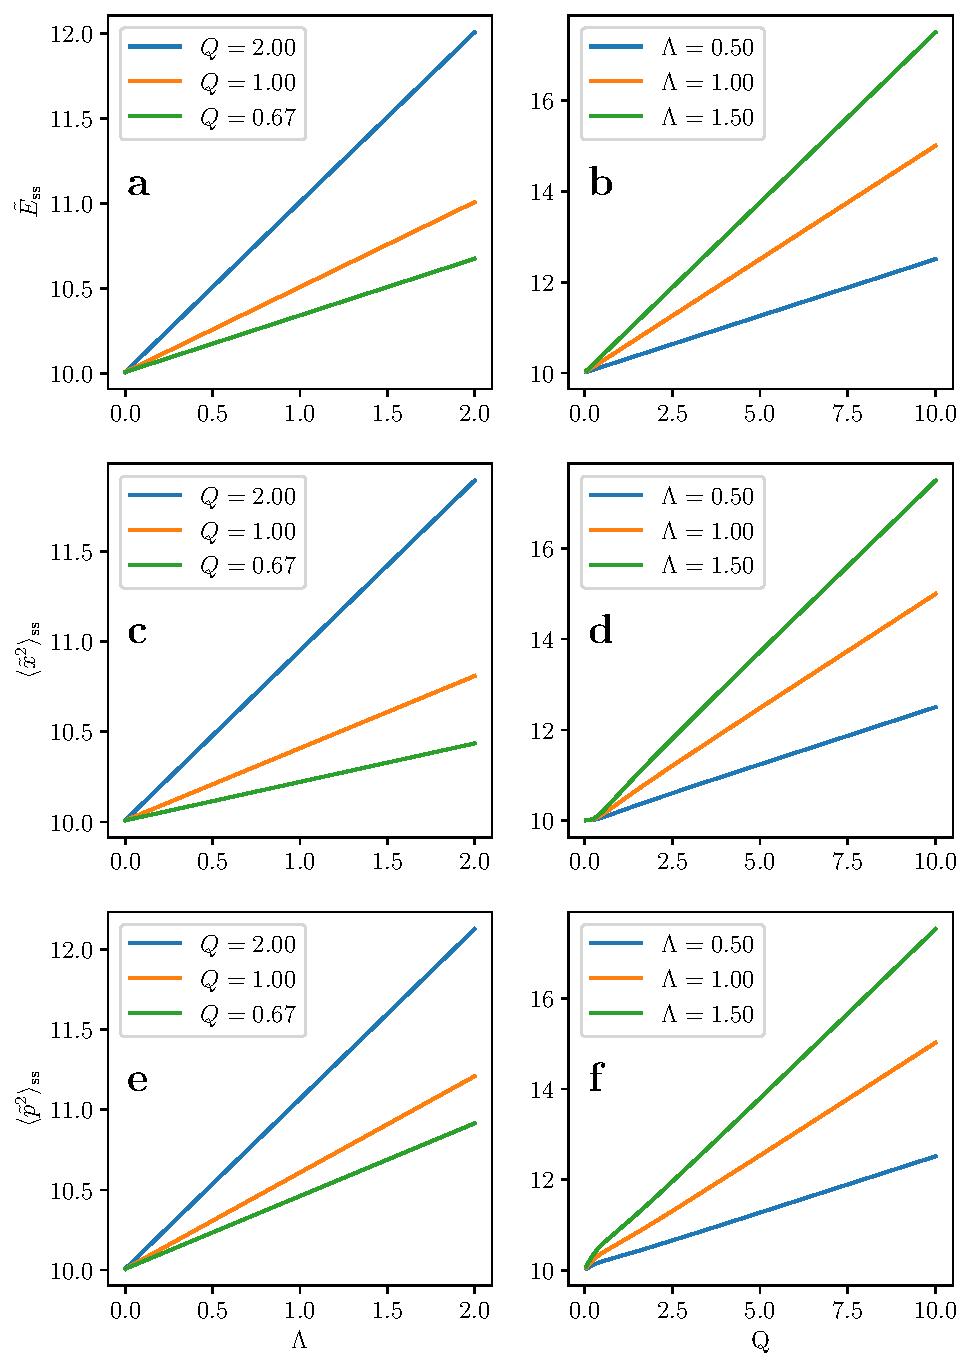
\includegraphics[width=\textwidth]{measurement_result.pdf}
    \caption{ \small The top panels show Eq. \eqref{eq:ess}, the middle panels show Eq. \eqref{eq:x2ss} and the bottom panels show Eq. \eqref{eq:p2ss}. All plots use the parameters $k_\mathrm{B}T = 10$ and $\omega = \hbar = 1$. The left panels are plotted against $\lambda / \omega$ and with three different values for $Q$, while the right panels are plotted against $Q$ and three different values of $\lambda$. }
    \label{fig:steady_state}
\end{figure}

Looking at panels \textbf{a} and \textbf{b} in Fig. \ref{fig:steady_state} one can see that a stronger measurement correlates to the system steady state increasing in energy, as does it for an increasing quality factor. Both also affect the system linearly. Thus, by continuously measuring the system we add energy into it, which make the steady state higher in energy than what the thermal effects from the bath would otherwise place it. That is, if we do not perform any measurement the system would be stable at around $\nbar + 1/2$ which for the parameters used here would give $\expval{\tilde{E}} \approx 10\hbar\omega$

We now consider a feedback mechanism on the oscillator described by Eq. \eqref{eq:masterFeed} which is a linear feedback scheme. Solving for the same EOM as before we obtain
\begin{align}
    \dt \expval{x^2} &= -\left(\gamma + \frac{4\im{f}}{\sqrt{2 m \omega \hbar}}\right) \expval{x^2} - \frac{1}{m} \expval{\acomm{x}{p}} + \frac{\gamma \hbar}{m \omega} (\nbar + 1/2) - \frac{1}{4\lambda m \omega \hbar} \re{f}^2,\\
    \dt \expval{p^2} &=  -\gamma \expval{p^2} + \left( m\omega^2 - \re{f} \sqrt{\frac{2m \omega}{\hbar}} \right)\expval{\acomm{x}{p}} + \gamma m \omega \hbar (\nbar + 1/2) + \lambda \hbar^2 + \frac{m \omega}{4 \lambda \hbar}\re{f}^2 ,\\
    \dt \expval{\acomm{x}{p}} &= \left(\frac{2}{\sqrt{2m \omega \hbar}}\im{f} - \gamma  \right)\expval{\acomm{x}{p}} + \left(2 m \omega^2 + 2 \sqrt{\frac{2 m \omega}{\hbar}}\re{f} \right) \expval{x^2} - \frac{2}{m} \expval{p^2} - \frac{\re{f} \im{f}}{2 \lambda \hbar}.
\end{align}
Performing the same change of variables as earlier with addition of 
\begin{equation}
    \re{\tilde{f}} = \sqrt{\frac{2 m}{\hbar \omega}} \re{f} \quad \text{and} \quad \im{\tilde{f}} = \frac{1}{\sqrt{2 m \omega \hbar}} \im{f}, 
\end{equation}
we can solve for the steady state. First we define
\begin{equation}
    D = 8m\lambda ( -\gamma ( -2\im{f} + \gamma ) (4\im{f} + \gamma)+ 8\im{f}\re{f} \omega - 4 (2\im{f} + \gamma)\omega^2 )\hbar
\end{equation}
then we can write the solutions as
\begin{multline}
    \expval{\tilde{x}^2} = \frac{1}{D} (\re{\tilde{f}} \omega (-2 \im{\tilde{f}} \gamma ( \re{\tilde{f}} - 2m \omega ) + \re{\tilde{f}} (\gamma^2 - 2 \re{\tilde{f}} \omega) ) \\ -8m (\nbar + 1/2)\gamma \omega(-2\im{\tilde{f}}\gamma + \gamma^2) - 2(\re{\tilde{f}}- 2\omega)\omega )\hbar
\end{multline}
\begin{multline}
    \expval{\tilde{p}^2} = \frac{1}{D} (\re{\tilde{f}} \omega ( -2 \re{\tilde{f}}^3 + \re{\tilde{f}} ( \im{\tilde{f}}(2 + 4m) - \gamma )(4 \im{\tilde{f}} + \gamma) \\- 2( \re{\tilde{f}}^2 + 2 \im{\tilde{f}} m (4 \im{\tilde{f}} + \gamma) ) \omega ) \\- 8m(\nbar + 1/2) \gamma \lambda ( -8 \im{\tilde{f}}^2 + 2 \im{\tilde{f}} \gamma + \gamma^2 - 2 (\re{\tilde{f}} - 2 \omega)(\re{\tilde{f}} + \omega) ) \hbar
    ) 
\end{multline}
\begin{multline}
    \expval{\acomm{\tilde{x}}{\tilde{p}}} = \frac{1}{D} (\re{\tilde{f}} \omega ( -8 \im{\tilde{f}}^2 m \gamma + \re{\tilde{f}} \gamma (\re{\tilde{f}} + 2 \omega) \\+ \im{\tilde{f}} (-2 m \gamma^2 + 4 \re{\tilde{f}} \omega) ) - 8 m (\nbar + 1/2) \gamma \lambda (\re{\tilde{f}} \gamma - 4 \im{\tilde{f}} \omega) \hbar
    )
\end{multline}